\documentclass[
    a4paper,          % Tamanho da folha A4
    12pt,             % Tamanho da fonte 12pt
    chapter=TITLE,    % Todos os capitulos devem ter caixa alta
    % section=TITLE,    % Todas as secoes devem ter caixa alta somente na primeira letra
    % subsection=TITLE, % Todas as subsecoes devem ter caixa alta somente na primeira letra
    oneside,          % Usada para impressao em apenas uma face do papel
    english,          % Hifenizacoes em ingles
    spanish,          % Hifenizacoes em espanhol
    brazil,           % Ultimo idioma eh o idioma padrao do documento
    fleqn             % Comente esta linha se quiser centralizar as equacoes. Comente também a linha 65 abaixo
]{lib/abntex2}

% Para utilizar este template siga o tutorial disponível em http://www.biblioteca.ufc.br/wp-content/uploads/2015/09/tutorial-sharelatex.pdf

%%%%%%%%%%%%%%%%%%%%%%%%%%%%%%%%%%%%%%%%%%%%%%%%%%%%%%%
%% Você deve criar uma conta no Overleaf. Depois,    %%
%% vá nas opções no canto esquerdo superior da tela  %%
%% e clique em "Copiar Projeto". Dê um novo nome pa- %%
%% ra o projeto.                                     %%
%%                                                   %%
%% Os principais desenvolvedores deste template são: %%
%%                                                   %%
%%            Ednardo Moreira Rodrigues              %%
%%       (Doutor em Engenharia Elétrica - UFC)       %%
%%(Coord. do Grupo de Astronomia da Seara da Ciência)%%
%%                      &                            %%
%%            Alan Batista de Oliveira               %%
%%           (Engenheiro Eletricista - UFC)          %%
%%                                                   %%
%% Consultoria Bibliotecária                         %%
%%                                                   %%
%%  Versão 2016 - ShareLaTeX:                        %% 
%%                                                   %%
%% - Francisco Edvander Pires Santos;                %%
%% - Juliana Soares Lima;                            %%
%% - Izabel Lima dos Santos;                         %%
%% - Kalline Yasmin Soares Feitosa;                  %%
%% - Eliene Maria Vieira de Moura.                   %%
%%                                                   %% 
%%  Versão 2019 - Overleaf:                          %%
%%                                                   %%
%%  Biblioteca de Ciências Humanas:                  %%
%% - Francisco Edvander Pires Santos;                %%
%% - Juliana Soares Lima;                            %%
%% - Eliene Maria Vieira de Moura;                   %%
%% - Edmundo Moreira de Sousa Filho.                 %%
%%                                                   %%
%% Biblioteca da FEAAC:                              %%
%% - Izabel Lima dos Santos;                         %%
%% - Kalline Yasmin Soares Feitosa;                  %%
%% - Kleber Lima dos Santos.                         %%
%%                                                   %%
%%  Biblioteca do Curso de Física:                   %%
%% - Aline Rodrigues de Lima Mendes;                 %%
%% - Maria de Jesus Silva dos Santos.                %%
%%                                                   %%
%%  Biblioteca Central do Campus do Pici:            %%
%% - Raquel da Silva Nascimento.                     %%
%% - Felipe Ferreira da Silva                        %%
%%                                                   %%
%% Colaboradores                                     %%
%%                                                   %%
%% -Andrei Bosco Bezerra Torres                      %% 
%% (Professor - Sistemas e Mídias Digitais -         %%
%% Instituto Universidade Virtual - UFC)             %%
%% Tiago Alves Lima                                  %% 
%% (Aluno de Mestrado em Eng. Elétrica)              %%
%%                                                   %%
%% Grande parte do trabalho foi adaptado do template %%
%% da UECE elaborado por:                            %%
%% Thiago Nascimento  (UECE)                         %%
%% Project available on:                             %%
%% https://github.com/thiagodnf/uecetex2             %%
%%                                                   %%
%% "Dúvidas, esclarecimentos ou sugestões podem ser  %%
%% enviadas para o seguinte e-mail:                  %%
%%                                                   %%
%%             atendimentobch@ufc.br                 %%
%%                                                   %%
%% As últimas atualizações estão descritas no inicio %%
%% do arquivo "README.md".                           %%
%%                                                   %%
%%%%%%%%%%%%%%%%%%%%%%%%%%%%%%%%%%%%%%%%%%%%%%%%%%%%%%%

\newcommand{\ctext}[3][RGB]{
  \begingroup
  \definecolor{color}{#1}{#2}\sethlcolor{color}
  \hl{#3}
  \endgroup
}

\newcommand{\qbox}[1]{\ctext[RGB]{180, 180, 250}{#1}}
\newcommand\sbullet[1][.7]{\mathbin{\vcenter{\hbox{\scalebox{#1}{$\bullet$}}}}}

\usepackage{etoolbox}
\usepackage{titlesec}
\usepackage{listofitems}
\usepackage{xstring}

\usepackage[table,xcdraw]{xcolor}
\usepackage{nicematrix}
\usepackage{soul}
\usepackage[most]{tcolorbox}
\usepackage{placeins}
\usepackage{hhline}
% \usepackage{fontspec}
% Importações de pacotes
\usepackage[T1]{fontenc}                            % Codificação da fonte em 8 bits
\usepackage{graphicx}                               % Inserir figuras
\usepackage{amsfonts, amssymb, amsmath}             % Fonte e símbolos matemáticos
\usepackage{booktabs}                               % Comandos para tabelas
\usepackage{verbatim}                               % Texto é interpretado como escrito no documento
\usepackage{multirow, array}                        % Múltiplas linhas e colunas em tabelas
\usepackage{indentfirst}                            % Endenta o primeiro parágrafo de cada seção.
\usepackage{listings}                               % Utilizar codigo fonte no documento

% \usepackage{microtype}                              % Para melhorias de justificação?
\usepackage[portuguese,ruled,lined]{algorithm2e}    % Escrever algoritmos
\usepackage{algorithmic}                            % Criar Algoritmos  
%\usepackage{float}                                 % Utilizado para criação de floats
\usepackage{amsgen}
\usepackage{lipsum}                                 % Usar a simulação de texto Lorem Ipsum
%\usepackage{titlesec}                              % Permite alterar os títulos do documento
\usepackage{tocloft}                                % Permite alterar a formatação do Sumário
\usepackage{etoolbox}                               % Usado para alterar a fonte da Section no Sumário
\usepackage[noredefwarn,nogroupskip,nonumberlist]{glossaries}   % Permite fazer o glossario. A apcao "sort=use" faz com que as siglas aparecam na lista conformse sao usadas no texto.

\usepackage[format=plain,justification=justified,skip=0pt,singlelinecheck = false,labelsep=colon]{ caption}            % Altera o comportamento da tag caption. Algumas opcoes do caption so podem ser alternada no arquivo "antex2.cls, linhas 334 a 348.

\usepackage{csquotes}

\usepackage[style=abnt]{biblatex}
\addbibresource{3-pos-textuais/referencias.bib}

% \usepackage{natbib}
% \usepackage[alf, abnt-emphasize=bf, recuo=0cm, abnt-etal-cite=2, abnt-etal-list=0, abnt-etal-text=it]{lib/ufcTexCite}  % Citações padrão UFC/ABNT NBR 6023 de 2018
% \usepackage[bottom]{footmisc}                      % Mantém as notas de rodapé sempre na mesma posição
%\usepackage{times}                                 % Usa a fonte Times
%%%%%%%%%%%%%%%%%%% AVISO %%%%%%%%%%%%%%%%%%%%%%%%%%%%%%%%%%%%%%%%
%descomente as duas linhas abaixo para alterar o texto de Times New Roman para Arial:

% \usepackage{helvet}
% \renewcommand{\familydefault}{\sfdefault}  % Usa a fonte Arial              
%%%%%%%%%%%%%%%%%%%%%%%%%%%%%%%%%%%%%%%%%%%%%%%%%%%%%%%%%%%%%%%%%%

\usepackage{mathptmx}         % Usa a fonte Times New Roman			%\usepackage{lmodern}         % Usa a fonte Latin Modern
%\usepackage{subfig}          % Posicionamento de figuras
%\usepackage{scalefnt}        % Permite redimensionar tamanho da fonte
%\usepackage{color, colortbl} % Comandos de cores
%\usepackage{lscape}          % Permite páginas em modo "paisagem"
%\usepackage{ae, aecompl}     % Fontes de alta qualidade
%\usepackage{picinpar}        % Dispor imagens em parágrafos
%\usepackage{latexsym}        % Símbolos matemáticos
%\usepackage{upgreek}         % Fonte letras gregas
\usepackage{appendix}         % Gerar o apendice no final do documento
\usepackage{paracol}          % Criar paragrafos sem identacao
\usepackage{lib/ufcTex}	      % Biblioteca com as normas da UFC para trabalhos academicos
\usepackage{pdfpages}         % Incluir pdf no documento
\usepackage{amsmath}          % Usar equacoes matematicas

\makeglossaries % Organiza e gera a lista de abreviaturas, simbolos e glossario
\makeindex      % Gera o Indice do documento         

\renewcommand{\labelitemi}{\textendash} %Altera os marcadores de itemize para 





\newcommand*{\monthname}[1]{%
  \ifcase#1
  \or
  jan.%
  \or
  fev.%
  \or
  mar.%
  \or
  abr.%
  \or
  maio%
  \or
  jun.%
  \or
  jul.%
  \or
  ago.%
  \or
  set.%
  \or
  oct.%
  \or
  nov.%
  \or
  dez.%
  \fi
}

\newcommand{\removezero}[1]{%
\StrMid{#1}{1}{1}[\zero]%
\StrMid{#1}{2}{3}[\inte]%
\ifthenelse{\equal{0}{\zero}}{\inte}{#1}%
}
\newcommand{\usedate}[1]{%
\def\x{#1}%
\setsepchar[.]{-}%
\readlist\datee{\x}%
{\removezero{\datee[2]} \monthname{\datee[3]} \datee[1]}%
}

\DeclareCaptionStyle{mystyle}
  {format=plain,%
    textformat=period,
    justification=RaggedRight,
    singlelinecheck=true,
  }% all captions are left aligned

\DeclareCaptionStyle{singlelinecentered}
  [justification=Centering]% centered if single line and no `singlelinecheck=false`
  {style=mystyle}% other captions are left aligned

\DeclareCaptionStyle{singlelineraggedleft}
  [justification=RaggedLeft]% right aligned if single line and no `singlelinecheck=false`
  {style=mystyle}% other captions are left aligned

\newcommand{\subsubsectionm}[1]{\subsubsection{\underline{#1}}}

\setlength{\mathindent}{0pt} %Complementa o alinhamento de equações para totalmente a esquerda.

\trabalhoacademico{tccgraduacao}

\ehqualificacao{nao}

\removerbordasdohyperlink{sim} 

\cordohyperlink{nao}

%%%%%%%%%%%%%%%%%%%%%%%%%%%%%%%%%%%%%%%%%%%%%%%%%%%%%
%%         Informacao sobre a instituicao          %%
%%%%%%%%%%%%%%%%%%%%%%%%%%%%%%%%%%%%%%%%%%%%%%%%%%%%%

\ies{Universidade Federal do Ceará}
\iessigla{UFC}
\centro{Campus Quixadá}
% \centro{Centro de Xxxxxxxx}
% \departamento{Departamento de Xxxxxxxxx}

%%%%%%%%%%%%%%%%%%%%%%%%%%%%%%%%%%%%%%%%%%%%%%%%%%%%%
%%        Informacao para TCC de Graduacao         %%
%%%%%%%%%%%%%%%%%%%%%%%%%%%%%%%%%%%%%%%%%%%%%%%%%%%%%

\graduacaoem{Ciência da computação}
\habilitacao{bacharel} % Ou licenciado(a)

% AVISO: Caso necessario alterar o texto de apresenta-
% cao da Especializacao, ir a pasta "lib", arquivo 
% "ufctex.sty" na linha 502.


%%%%%%%%%%%%%%%%%%%%%%%%%%%%%%%%%%%%%%%%%%%%%%%%%%%%%
%%     Informacao para TCC de Especializacao       %%
%%%%%%%%%%%%%%%%%%%%%%%%%%%%%%%%%%%%%%%%%%%%%%%%%%%%%

% \especializacaoem{Yyyyyyyyy}

% AVISO: Caso necessario alterar o texto de apresenta-
% cao da Especializacao, ir a pasta "lib", arquivo 
% "ufctex.sty" na linha 507.

%%%%%%%%%%%%%%%%%%%%%%%%%%%%%%%%%%%%%%%%%%%%%%%%%%%%%
%%         Informacao para Dissertacao             %%
%%%%%%%%%%%%%%%%%%%%%%%%%%%%%%%%%%%%%%%%%%%%%%%%%%%%%

% \programamestrado{Programa de Pós-Graduação em Xxxxxxx}
% \nomedomestrado{Mestrado Acadêmico em Xxxxxxx}
% \mestreem{Engenharia Xxxxxx}
% \areadeconcentracaomestrado{Engenharia Xxxxxx}

% AVISO: Caso necessario alterar o texto de apresenta-
% cao da dissertacao, ir a pasta "lib", arquivo 
% "ufctex.sty" na linha 511.

%%%%%%%%%%%%%%%%%%%%%%%%%%%%%%%%%%%%%%%%%%%%%%%%%%%%%
%%               Informação para Tese              %%
%%%%%%%%%%%%%%%%%%%%%%%%%%%%%%%%%%%%%%%%%%%%%%%%%%%%%

% \programadoutorado{Programa de Pós-Graduação em Xxxxxx}
% \nomedodoutorado{Doutorado em Xxxxxxx}
% \doutorem{Engenharia Xxxxxx}
% \areadeconcentracaodoutorado{Engenharia Xxxxxxx}

% AVISO: Caso necessario alterar o texto de apresenta-
% cao da tese, ir a pasta "lib", arquivo "ufctex.sty" 
% na linha 515.

%%%%%%%%%%%%%%%%%%%%%%%%%%%%%%%%%%%%%%%%%%%%%%%%%%%%%
%%      Informacoes relacionadas ao trabalho       %%
%%%%%%%%%%%%%%%%%%%%%%%%%%%%%%%%%%%%%%%%%%%%%%%%%%%%%

\autor{Francisco Fagner Ferreira Mesquita}
\titulo{Uma ferramenta para o ensino de algoritmos de análise sintática}
\data{2024}
\local{Quixadá}

% Exemplo: \dataaprovacao{01 de Janeiro de 2012}
\dataaprovacao{xx/xx/xxxx.}

%%%%%%%%%%%%%%%%%%%%%%%%%%%%%%%%%%%%%%%%%%%%%%%%%%%%%
%%           Informação sobre o Orientador         %%
%%%%%%%%%%%%%%%%%%%%%%%%%%%%%%%%%%%%%%%%%%%%%%%%%%%%%

\orientador{Prof. Dr. João Marcelo Uchôa de Alencar}
\orientadories{Universidade Federal do Ceará (UFC)}
\orientadorcentro{Centro de Ciências e Tecnologia (CCT)}
\orientadorfeminino{nao} % Coloque 'sim' se for do sexo feminino

%%%%%%%%%%%%%%%%%%%%%%%%%%%%%%%%%%%%%%%%%%%%%%%%%%%%%
%%          Informação sobre o Coorientador        %%
%%%%%%%%%%%%%%%%%%%%%%%%%%%%%%%%%%%%%%%%%%%%%%%%%%%%%

% Deixe o nome do coorientador em branco para remover do documento

% \coorientador{Prof. Dr. Xxxxxx (Se houver)}
% \coorientadories{Universidade Coorientador (SIGLA)}
% \coorientadorcentro{Centro do Coorientador (SIGLA)}
% \coorientadorfeminino{nao} % Coloque 'sim' se for do sexo feminino

%%%%%%%%%%%%%%%%%%%%%%%%%%%%%%%%%%%%%%%%%%%%%%%%%%%%%
%%              Informação sobre a banca           %%
%%%%%%%%%%%%%%%%%%%%%%%%%%%%%%%%%%%%%%%%%%%%%%%%%%%%%

% Atenção! Deixe em branco o nome do membro da banca para remover da folha de aprovacao

% Exemplo de uso:
% \membrodabancadois{Prof. Dr. Fulano de Tal}
% \membrodabancadoisies{Universidade Federal do Ceará - UFC}


\membrodabancadois{Prof. Dr. Xxxxxxx Xxxxxx Xxxxxxx}
\membrodabancadoiscentro{Faculdade de Filosofia Dom Aureliano Matos (FAFIDAM)}
\membrodabancadoisies{Universidade do Membro da Banca três (SIGLA)}
\membrodabancatres{Prof. Dr. Xxxxxxx Xxxxxx Xxxxxxx}
\membrodabancatrescentro{Centro de Ciências e Tecnologia (CCT)}
\membrodabancatresies{Universidade do Membro da Banca quatro (SIGLA)}
\membrodabancaquatro{Prof. Dr. Xxxxxxx Xxxxxx Xxxxxxx}
\membrodabancaquatrocentro{Centro de Ciências e Tecnologia (CCT)}
\membrodabancaquatroies{Universidade do Membro da Banca cinco (SIGLA)}
\membrodabancacinco{Prof. Dr. Xxxxxxx Xxxxxx Xxxxxxx}
\membrodabancacincocentro{Teste}
\membrodabancacincoies{Universidade do Membro da Banca seis (SIGLA)}
\membrodabancaseis{Prof. Dr. Xxxxxxx Xxxxxx Xxxxxxx}
\membrodabancaseiscentro{}
\membrodabancaseisies{Universidade do Membro da Banca sete (SIGLA)}
 

\begin{document}
    \imprimircapa
	\imprimirfolhaderosto{} 
	%\imprimirfichacatalografica{1-pre-textuais/ficha-catalografica}
	%\imprimirerrata{elementos-pre-textuais/errata}
	% \imprimirfolhadeaprovacao
	% \imprimirdedicatoria{1-pre-textuais/dedicatoria}
	% \imprimiragradecimentos{1-pre-textuais/agradecimentos}
	% \imprimirepigrafe{1-pre-textuais/epigrafe}
	% \imprimirresumo{1-pre-textuais/resumo}
	% \imprimirabstract{1-pre-textuais/abstract}
	% \renewcommand*\listfigurename{Lista de Figuras} %Se você comentar esta linha o título da lista fica: LISTA DE ILUSTRAÇÕES
	% \imprimirlistadeilustracoes
	% \imprimirlistadetabelas
	% \imprimirlistadequadros
	% \imprimirlistadealgoritmos
	% \imprimirlistadecodigosfonte
	% \imprimirlistadeabreviaturasesiglas
	% \imprimirlistadesimbolos{1-pre-textuais/lista-de-simbolos}   
	\imprimirsumario

	\setcounter{table}{0}% Deixe este comando antes da primeira tabela.
	
	%Elementos textuais
	\textual
	\chapter{Introdução}
\label{cap:introducao}

Um compilador é uma ferramenta usada para compilar código-fonte de uma linguagem de alto nível para código de máquina. Esse processo é feito em várias fases, as três primeiras fases do processo de compilação podem ser definidas como análise léxica, análise sintática e checagem de tipo, elas são chamadas coletivamente de \textit{front-end} do compilador \cite{mogensen2024introduction}.

A fase de análise léxica gera \textit{tokens} que são usados pela fase de análise sintática para validar que a entrada segue a estrutura da gramática da linguagem alvo e gerar uma árvore sintática para ser usada pelas próximas fases da compilação \cite{thain2020introduction}.

O programa que realiza a análise sintática é chamado de analisador sintático ou \textit{parser}. Os \textit{parsers} podem ser classificados em dois tipos, \textit{bottom-up} (ou ascendente) que funciona reduzindo os \textit{tokens} a produções da gramática e \textit{top-down} (ou descendente) que segue o caminho oposto do \textit{parser bottom-up} tentando encontrar produções correspondentes a estrutura da \textit{string} de entrada comparando-a com as produções da gramática \cite{cooper2022engineering}.

A disciplina de compiladores está presente em muitas grades curriculares de cursos de ciência da computação e dentro dessa disciplina são ensinados vários algoritmos de análise sintática, no entanto, aprender o funcionamento desses algoritmos é uma tarefa difícil para os alunos, assim como também é difícil para os professores ensinarem esse assunto \cite{sangal2018pavt}.

Ferramentas criadas para o ensino de conteúdos sobre construção de compiladores como análise sintática usando elementos visuais têm uma resposta positiva dos alunos que usaram as ferramentas. Essas ferramentas podem auxiliar na compreensão do conteúdo não só através das instruções mostradas na visualização do funcionamento dos algoritmos, mas também por oferecer respostas instantâneas que podem ser usadas pelos estudantes como correção sobre os resultados dos algoritmos que podem ser difíceis de se construir manualmente \cite{10.1145/3002136}.

A instabilidade na rede disponível no campus Quixadá da \gls{ufc} é algo recorrente que pode atrapalhar o roteiro normal das aulas e impedir que os alunos concluam tarefas propostas em aula \cite{perez2023impact}. O uso de aplicações desenvolvidas para \textit{web} nas aulas é afetado por eventuais falhas na rede local do campus e em relação a isso uma aplicação \textit{offline} desenvolvida para \textit{desktop} tem a vantagem de poder ser acessada independente do acesso à internet \cite{holzer2012mobile}. Utilizar o servidor local do campus para hospedar a ferramenta também pode melhorar a disponibilidade do software já que o servidor local do campus sofre instabilidade que a rede local.

Muitos alunos entram na vida universitária estando em situação de vulnerabilidade econômica e sem recursos necessários como computadores para acompanhar o conteúdo do curso, algo que faz alusão a essa realidade é a disponibilização de bolsas de inclusão feita pela UFC durante o período da pandemia para auxiliar na aquisição de computadores \cite{povo_ufc_2020}. Assim, a utilização de uma aplicação \textit{mobile} no lugar de uma aplicação \textit{desktop} nas aulas seria mais inclusiva.

Apesar da desvantagem citada nos parágrafos anteriores, uma ferramenta \textit{web} tem outras vantagens notáveis como não haver a necessidade de instalação do \textit{software} para acessá-lo e a facilidade de integração com plataformas como o \textit{Moodle}\footnote{https://moodle2.quixada.ufc.br/} \cite{desai_web_2022}.

Todas as abordagens de desenvolvimento citadas têm suas vantagens e desvantagens, mas não é preciso  escolher uma abordagem em detrimento da outra. \textit{Frameworks} modernos como \textit{Tauri}\footnote{https://tauri.app/} e \textit{Capacitor}\footnote{https://capacitorjs.com/} permitem que uma única base de código seja usada para desenvolver software para diferentes plataformas, graças a isso, torna-se possível o desenvolvimento multi-plataforma da ferramenta proposta nesse trabalho \cite{shevtsiv2021cross}.

\section{Objetivos}
O objetivo desse trabalho é criar uma ferramenta multi-plataforma que possa ser acessada \textit{offline} e \textit{online} sendo hospedada local remotamente e que por meio de uma mistura de elementos visuais e textuais ajude a entender como funcionam os algoritmos de análise sintática e quais os processos necessários para obter a saída de cada passo dos algoritmos.

Esse trabalho tem os seguintes objetivos específicos:
\begin{itemize}[label=$\sbullet$]
    \item Criar a ferramenta usando \textit{Svelte}\footnote{https://svelte.dev/}.
    \item Oferecer uma forma de visualização dos algoritmos CLR, SLR e LL(1).
    \item Oferecer uma versão \textit{web} da ferramenta
    \item Oferecer uma versão \textit{desktop} da ferramenta
    \item Oferecer uma versão \textit{mobile} da ferramenta
    \item Integração da ferramenta com a plataforma \textit{Moodle}.
    \item Validar a ferramenta fazendo uma avaliação com alunos.
\end{itemize}


	\chapter{Fundamentação teórica}
\label{cap:fundamentacao-teorica}

Neste capítulo apresentaremos os conceitos centrais que serviram como base e guia para a elaboração deste trabalho. Ao início é falado sobre o conhecimento básico sobre compiladores, depois sobre o \textit{framework} utilizado para construção da ferramenta e por fim, sobre a tecnologia usada para fazer a integração com o \textit{Moodle}.

\section{Compiladores}
Programas que são executados em computadores são escritos no que é chamada de linguagem de máquina que usa comandos simples que são interpretados pela máquina. Escrever em linguagem de máquina é uma tarefa passível de erro e cansativa, e por essa razão foram criados os compiladores. Os compiladores traduzem linguagens de alto nível em linguagem de máquina e indicam erros cometidos pelos programadores no código-fonte \cite{mogensen2024introduction}.

\subsection{Fases do compilador}
As fases de um compilador podem ser divididas de várias formas. Os trabalhos de \textcite{cooper2022engineering,mogensen2024introduction, thain2020introduction} dão suas definições das fases de um compilador, mas para esse trabalho será seguida a definição de \textcite{thain2020introduction}. 

\begin{figure}[ht]
    \captionsetup{width=16cm}
    \Caption{\label{fig:compfases}Fases de um compilador UNIX}
    \tcbox[left=0cm, right=0cm, top=0cm, bottom=0cm,center]{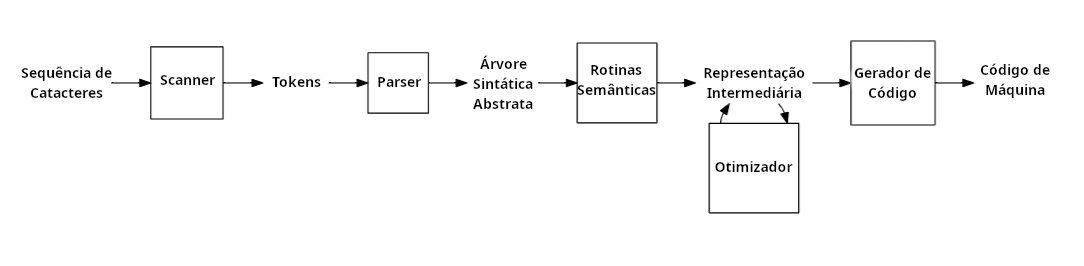
\includegraphics[width=15.6cm]{figuras/compfases.png}}{
    \Fonte{adaptada de \textcite{thain2020introduction}.}}
\end{figure}

\subsubsection{Análise Léxica}
Na fase de análise léxica, o \textit{scanner}, também chamado de \textit{tokenizer}, consome texto simples de um programa e agrupa os caracteres individuais em sequências chamadas de \textit{tokens}. Esse processo funciona de forma parecida com agrupar letras para formar palavras da linguagem natural, esse agrupamento é feito usando expressões regulares implementadas através de autômatos.

\subsubsection{Análise Sintática}
Análise de sintática será o foco do trabalho sendo discutida de forma mais aprofundada nas próximas seções. A fase de análise sintática da compilação rearranja os \textit{tokens} gerados pela fase de análise léxica, gerando assim uma estrutura chamada árvore sintática. Árvores sintáticas são estruturas de árvore como diz o nome, as folhas dessa árvore são os \textit{tokens} e a leitura em ordem da árvore dá a sequência de \textit{tokens} do texto de entrada dado ao analisador sintático. Ao construir a árvore sintática, o analisador sintático também checa se há erros de sintaxe no texto de entrada.

\subsubsection{Análise semântica}
Na fase de análise semântica, as rotinas semânticas percorrem a árvore sintática e buscam significado na entrada a partir das regras da gramática e da relação entre os elementos da entrada. Depois das rotinas semânticas, a árvore de análise sintática é convertida em uma representação intermediária que é uma versão simplificada de \textit{assembly} que permite uma análise detalhada.

\subsubsection{Otimização}
Na fase de otimização, otimizadores são aplicados na representação intermediária para tornar o programa mais rápido, menor e eficiente. Normalmente os otimizadores recebem uma entrada em formato de representação intermediária e retornam um resultado no mesmo formato para que todos os otimizadores possam ser aplicados de forma independente e em qualquer ordem.

\subsubsection{Geração de código}
Na fase de geração de código, o gerador de código consome a representação intermediária otimizada e a transforma em um programa em \textit{assembly} concreto. Para otimizar o uso dos registradores físicos limitados e gerar instruções de montagem de maneira eficiente, o gerador de código precisa executar as tarefas de alocação de registradores, seleção de instruções e sequenciamento de instruções.

\section{Analisadores Sintáticos Descendentes}
\textcite{cooper2022engineering,mogensen2024introduction, thain2020introduction} falam sobre analisadores sintáticos descendentes, mas para esse trabalhos será seguida a definiçã de \textcite{thain2020introduction}. Analisadores sintáticos descendentes, também chamados \textit{parsers top-down}, são métodos de análise sintática que iniciam a análise a partir do símbolo inicial da gramática. Eles fazem comparações entre os \textit{tokens} do texto de entrada e os símbolos da gramática para encontrar a produção que deve ser escrita no lugar dos símbolos da gramática. Essas comparações são feitas até sobrar apenas símbolos terminais, esses símbolos terminais devem coincidir com a sequência de \textit{tokens} da entrada caso contrário será considerado um erro.

\subsection{Descendentes Recursivos}
O conjunto de gramáticas que pode ser analisados usando algoritmos usando apenas um não terminal e o próximo símbolo da entrada é chamado conjunto de gramáticas LL(1). Uma das formas de fazer a análise dessas gramáticas é usando o analisador sintático descendente recursivo que usa funções recursivas para cada não terminal para processar a entrada. É um algoritmo que funciona como uma forma recursiva dos analisadores sintáticos LL(1) que já são tratados nesse trabalho, além disso, esse algoritmo não segue estruturas fixas e determinísticas, por isso não será abordado na ferramenta.

\subsection{Analisadores Sintáticos LL(1)} 
% \ctext[RGB]{180, 250, 180}{Escrever mais detalhado sobre LL(1)} \newline
Analisadores sintáticos LL(1) são um tipo de analisador sintático descendente, esses analisadores sintáticos levam em consideração um \textit{lookahead} que nesse algoritmo é o símbolo inicial do lado direito das produções. O \textit{lookahead} é usado para decidir qual produção deve ser escrita, por essa razão apenas gramaticas não ambíguas podem ser analisadas pelos analisadores sintáticos LL(1).

O conjunto dos símbolos iniciais das produções de uma gramática é chamado conjunto \textit{first}, a construção desse conjunto pode ser feita seguindo o Algoritmo \ref{alg:first}. As definições dos algoritmos foram tiradas do trabalho de \textcite{thain2020introduction}.

\begin{algorithm}[htp]
    \caption{First}\label{alg:first}
    \Input{Gramática G, simbolo X }
    \Output{Conjunto first}
    \Inicio{
        first = \selectlanguage{brazil}$\{\}$\\
        \Switch{X}{
            \Case {Terminal}{
                first = \{X\}
            } 
            \Casex{Não terminal}{
                \Repeat{não haja mais mudanças}{
                    \ForEach{regra \selectlanguage{brazil}$X \rightarrow Y_1Y_2...Y_k$\selectlanguage{brazil} na Gramática G}{
                        \Ifx {a está em First($Y_1$) ou a está em First($Y_n$) e \selectlanguage{brazil}$Y_1.. Y_{n-1} \Rightarrow \epsilon$} {Adicionar a ao first}            \Ifx{$Y_1...Y_k \Rightarrow \epsilon$}{
                        Adicionar \selectlanguage{brazil}$\epsilon$\selectlanguage{brazil} ao first
                        }
                    }
                }
            }
        }
        \Return{first}
    }
\end{algorithm}
\selectlanguage{brazil}

O conjunto \textit{follow} é o conjunto de símbolos terminais da gramática que podem ocorrer depois de qualquer uma das derivações de um não terminal \selectlanguage{brazil}$A$\selectlanguage{brazil}, o conjunto também inclui o símbolo \$ usado para se referir ao fim da \textit{string}. Esse conjunto é usado no analisador LL para lidar com produções que derivam uma \textit{string} vazia. A construção do conjunto \textit{follow} pode ser feita seguindo o Algoritmo \ref{alg:follow}.

Uma tabela de análise sintática LL(1) pode ser usada para determinar as regras a serem usadas na análise de uma trada para todas as combinações de não terminais e \textit{tokens} da entrada. A construção dessa tabela pode ser feita usando os conjuntos de \textit{first} e \textit{follow} usando o Algoritmo \ref{alg:lltable}.

Tendo a tabela de análise sintática LL(1) em mãos, é possível fazer a análise de uma sequência de \textit{tokens} usando uma \textit{stack}. O Algoritmo \ref{alg:lltparse} mostra a análise sintática usando a tabela. 

\begin{algorithm}[htp]
    \caption{Follow}\label{alg:follow}
    \Input{Gramática G}
    \Output{Conjunto follow}
    \Inicio{
        follow = \{\} \\
        follow(S) = \{\$\} onde S é o símbolo inicial.\\
        \Repeat{ até não houver mais mudanças}{
        \Ifx {A → \selectlanguage{brazil}$\alpha B \beta$\selectlanguage{brazil} }{
        adiciona First($\beta$) (exceto \selectlanguage{brazil}$\epsilon$) follow(B).}
        \Ifx {A → \selectlanguage{brazil}$\alpha B$\selectlanguage{brazil} ou First($\beta$) contém \selectlanguage{brazil}$\epsilon$} {
        adiciona follow(A) ao follow(B).}
        }

        \Return{follow}
    }
\end{algorithm}
\selectlanguage{brazil}

\section{Analisadores Sintáticos Ascendentes}
\textcite{cooper2022engineering,mogensen2024introduction, thain2020introduction} falam sobre analisadores sintáticos ascendentes, mas para esse trabalhos será seguida a definiçã de \textcite{thain2020introduction}. Os analisadores sintáticos ascendentes levam uma abordagem oposta aos analisadores sintáticos descendentes. Ao invés de começar com o símbolo inicial da gramática, os analisadores sintáticos ascendentes procuram sequências de \textit{tokens} que façam par com o lado direito das produções da gramática e substituem as sequências de \textit{tokens} pelo símbolo não terminal do lado esquerdo da produção. Esse processo é repetido até que toda a sequência de \textit{tokens} seja reescrita e apenas reste o símbolo inicial da gramática.

\subsection{Analisadores Sintáticos SLR}
Há um conjunto de gramáticas que podem ser analisadas usando técnicas de \textit{shift-reduce} e um único \textit{lookahead}, esse conjunto de gramáticas pode ser chamado de LR(0). As ações de \textit{shift-reduce} são usadas para reduzir \textit{tokens} de uma entrada a não terminais, quando uma sequência de \textit{tokens} pode ser reduzida ao símbolo inicial da gramática a análise da entrada teve sucesso, caso contrário há um erro na entrada.

\begin{algorithm}[htp]
    \caption { Construção da tabela LL(1)}\label{alg:lltable}
    
    \Input {Gramática G}
    \Output {Tabela M }
    \Inicio{
        \ForEach {regra A \selectlanguage{brazil}$\rightarrow \alpha$\selectlanguage{brazil} em G} {
            \ForEach {terminal \selectlanguage{brazil}$a$\selectlanguage{brazil} (exceto \selectlanguage{brazil}$\epsilon$) em First($\alpha$)} {
                adiciona A \selectlanguage{brazil}$\rightarrow \alpha$\selectlanguage{brazil} a \selectlanguage{brazil}$T [A, a]$.}
            \Ifx {$\epsilon$\selectlanguage{brazil} está em First($\alpha$)}
                {\ForEach {terminal b (incluindo \$) em Follow(A)}{
                adiciona A \selectlanguage{brazil}$\rightarrow \alpha$\selectlanguage{brazil} to \selectlanguage{brazil}$T [A, b]$.}}
        }
    }
\end{algorithm}
\selectlanguage{brazil}

\begin{algorithm}[htp]
\caption{Análise com tabela LL(1)}\label{alg:lltparse}
\Input{Gramática G com simbolo inicial P, tabela T}
\Inicio{
    cria uma stack S.\\
    monta \$\selectlanguage{brazil} e P em S.\\
    token c = o primeiro token na entrada.\\
    \While {S não está vazio} {
        token X = o topo de S. \\
        \Ifx {X faz par com c} {
            remova X de S.\\
            avança c para o proximo token\\
            repetir.}
        \Ifx {X é um terminal} {para com um erro.}
        \Ifx {T [X, c] aponta para a regra \selectlanguage{brazil}$X \rightarrow \alpha$}{
            remova X de S.\\
            monta os símbolos \selectlanguage{brazil}$\alpha$\selectlanguage{brazil} em S.\\
            repetir.}
        \Ifx {T [X, c] aponta para um estado de erro} {para com um erro.}
    }
}
\end{algorithm}
\selectlanguage{brazil}
Todas as ações de \textit{shift-reduce} possíveis podem ser calculadas para uma gramática construindo um autômato LR(0), que também pode ser chamado coleção de itens canônicos. Esse autômato guarda todas as possíveis posições de leitura das produções da gramática representadas por um ponto escrito no lado direito das produções.

As ações de \textit{shift-reduce} são definidas pelas transições do autômato e pela posição de leitura, caso uma transição seja feita com um terminal a ação será de \textit{shift}, caso uma transição seja feita com um não terminal a ação será de \textit{goto}, caso a posição de leitura esteja no fim da produção a ação será de \textit{reduce}. 

O Algoritmo \ref{alg:automaton} mostra como construir o autômato LR(0) com o auxílio do \textit{closure} mostrado no Algoritmo \ref{alg:closure}.

\begin{algorithm}[ht]
    \caption{Closure}\label{alg:closure}
    \Input{Gramática G, Estado S}
    \Inicio{
        \Repeat{não tenha itens a serem adicionados}{ 
            \ForEach {item da forma \selectlanguage{brazil}$A \rightarrow \alpha .X \beta$\selectlanguage{brazil} em S com \selectlanguage{brazil}$X \in NT$\selectlanguage{brazil} } {
                \ForEach{produção da forma \selectlanguage{brazil}$X \rightarrow \gamma \selectlanguage{brazil}$\selectlanguage{brazil} em G}{
                    adiciona uma produção da forma \selectlanguage{brazil}$X \rightarrow .\gamma$\selectlanguage{brazil} a S
                }
            }
        }
    }
\end{algorithm}
\selectlanguage{brazil}

Quando um símbolo não terminal produz um símbolo terminal, apenas um caminho para derivação é possível, já que um não terminal não pode ser derivado, no entanto, quando um não terminal produz outro não terminal, o não terminal produzido terá outras derivações. Por essa razão é preciso levar em consideração as produções dos não terminais que estão sob a posição de leitura dentro da produção de outro não terminal. \textit{Closure} é o nome dado a ação de completar os estados do autômato adicionando essas produções. 

\begin{algorithm}[ht]
    \caption{Construção do autômato LR(0)}\label{alg:automaton}
    \Input{Gramática G}
    \Output{Autômato LR(0)}
    \Inicio{
        cria um autômato m. \\
        estado s0 = \{P | para a produção do símbolo inicial \selectlanguage{brazil}$A \rightarrow \gamma$, P é uma produção da forma \selectlanguage{brazil}$A \rightarrow .\gamma$\selectlanguage{brazil} \}.\\
        closure(s0).\\
        adiciona s0 a m.\\
        conjunto de estados newStates = \{s0\}. \\
        \ForEach{estado s em newStates} {
            conjunto de estados temp = \{\}.\\
            \ForEach{símbolo a em \selectlanguage{brazil}$T\cup NT$}{
                estado s1 = \{\}.\\
                \ForEach{produção da forma \selectlanguage{brazil}$A \rightarrow \alpha . a \beta$\selectlanguage{brazil} em s}{
                    adiciona uma produção da forma \selectlanguage{brazil}$A \rightarrow \alpha a. \beta$\selectlanguage{brazil} em s1.\\
                }
                
                closure(s1).\\
                
                \Ifx{s1 não está em m}{ 
                    adiciona s1 a m.\\
                    adiciona a transição \selectlanguage{brazil}$\hat{\delta}(s, a)=\hat{\delta}(s, a)\cup\{s1\}$\selectlanguage{brazil} a m.\\
                    adiciona s1 a temp.
                }
            }
            newStates = temp
        }
        \Return{m}
    }
\end{algorithm}
%\FloatBarrier 
\selectlanguage{brazil}

Usando o autômato LR(0) podemos construir uma tabela de ações e \textit{goto} para facilitar o acesso a essas informações durante o processo de análise sintática. Essa pode ser calculada usando o Algoritmo \ref{alg:slrtable}.

A análise sintática do analisador sintático SLR pode ser feita usando a tabela de ações e \textit{goto} seguindo o Algoritmo \ref{alg:slrparsing}.
\begin{algorithm}[htp]
    \caption{Construção da tabela SLR}\label{alg:slrtable}
    \Input{Autômato LR(0)}
    \Inicio{
        tabela ACTION\\
        tabela GOTO\\
        \ForEach {estado s} {
            \ForEach {item da forma \selectlanguage{brazil}$A \rightarrow \alpha . a \beta$}{
                ACTION[s, a] = shift para o estado t de acordo com o autômato LR(0).}
            \ForEach {item da forma \selectlanguage{brazil}$A \rightarrow \alpha . B \beta$}{
                GOTO[s, B] = goto para o estado t de acordo com o autômato LR(0).}
            \ForEach {item da forma \selectlanguage{brazil}$A \rightarrow \alpha .$}{
                \ForEach{ terminal a em FOLLOW(A)}{
                    ACTION[s, a] = reduce pela regra \selectlanguage{brazil}$A \rightarrow \alpha$.
                }
            }
        }
        Todos os estados restantes são estados de erro.
    }
\end{algorithm}
%\FloatBarrier
\selectlanguage{brazil}


\subsection{Analisadores Sintáticos CLR}
O analisador sintático \textit{canonical} LR (CLR) é um analisador sintático descendente para gramáticas LR(1). O analisador sintático CLR usa o autômato LR(1) para construção da tabela de ações e \textit{goto}, esse autômato é parecido com o autômato LR(0), o que diferencia os dois é que todos os itens do autômato LR(1) tem uma anotação do conjunto de \textit{tokens} que podem aparecer depois desses itens. Esse conjunto é chamado \textit{lookahead}. 

\begin{algorithm}[htp]
    \caption{Analise com tabela SLR}\label{alg:slrparsing}
    \Input{Tabela de ações ACTION, Tabela goto GOTO}
    \Inicio{
        stack de estados S.\\
        monta S0 em S.\\
        token a = primeiro token da entrada.\\
        \While{verdade}{
        estado s = topo de S.\\
        \If {ACTION[s, a] for aceite}{
        analise completa.}
        \ElseIf {ACTION[s, a] for shift t}{
        monta estado t em S.\\
        token a = próximo token da entrada.}
        \ElseIf {ACTION[s, a] for reduce \selectlanguage{brazil}$A \rightarrow \beta$}{
        desmonta estados correspondentes a \selectlanguage{brazil}$\beta$\selectlanguage{brazil} de S.\\
        estado t = topo de S.\\
        monta GOTO[t, A] em S.}
        \Elsex{
        para com um erro.}
        }
    }
\end{algorithm}
\selectlanguage{brazil}

A construção do autômato LR(1) segue o mesmo algoritmo da construção do autômato LR(0) com algumas modificações. A primeira produção a ser adicionada no primeiro estado do autômato vai ser adicionada com o \textit{lookahead}, esse \textit{lookahead} tem \selectlanguage{brazil}$\$$\selectlanguage{brazil} como único elemento. Ao computar o \textit{closure} serão considerados dois casos:
\begin{itemize}[label=$\sbullet$]
    \item Para produções da forma \selectlanguage{brazil}$A \rightarrow \alpha . B \selectlanguage{brazil}$\selectlanguage{brazil} com \textit{lookahead} de \selectlanguage{brazil}$\{L\}$, deverão ser adicionadas novas produções da forma \selectlanguage{brazil}$B \rightarrow . \gamma$\selectlanguage{brazil} com \textit{lookahead} de \selectlanguage{brazil}$\{L\}$
    \item Para produções da forma \selectlanguage{brazil}$A \rightarrow \alpha.B\beta$, com \textit{lookahead} de \selectlanguage{brazil}$\{L\}$, deverão ser adicionadas novas produções da forma \selectlanguage{brazil}$B \rightarrow . \gamma$\selectlanguage{brazil} com \textit{lookahead} da seguinte forma:
    \begin{itemize}
        \item Se \selectlanguage{brazil}$\beta$\selectlanguage{brazil} não produz \selectlanguage{brazil}$\epsilon$, o \textit{lookahead} é \selectlanguage{brazil}$First(\beta)$.
        \item Se \selectlanguage{brazil}$\beta$\selectlanguage{brazil} produz \selectlanguage{brazil}$\epsilon$, o \textit{lookahead} é \selectlanguage{brazil}$First(\beta)\cup\{L\}$.
    \end{itemize}
\end{itemize}
\selectlanguage{brazil}

Com essas modificações chegamos aos algoritmos de \textit{closure} LR(1) e construção do autômato LR(1) que podem ser vistos nos algoritmos \ref{alg:closurelr1} e \ref{alg:automatonlr1} respectivamente.

\begin{algorithm}[ht]
    \caption{Closure LR(1)}\label{alg:closurelr1}
    \Input{Gramática G, Estado S}
    \Inicio{
        \Repeat{não tenha itens a serem adicionados}{ 
            \ForEach {item da forma \selectlanguage{brazil}$A \rightarrow \alpha . B$\selectlanguage{brazil} em S com lookahead de \{L\}$\selectlanguage{brazil}$ } {
                adiciona as produções da forma \selectlanguage{brazil}$B \rightarrow .\gamma$\selectlanguage{brazil} a S
                
            }
            \ForEach {item da forma \selectlanguage{brazil}$A \rightarrow \alpha . B \beta$\selectlanguage{brazil} em S com lookahead de \{L\}$\selectlanguage{brazil}$ } {
                \ForEach {item da forma $B \rightarrow \gamma$ em G }
                { 
                    \If{
                        $\beta$ não produz $\epsilon$
                    } {
                        adiciona uma produção da forma $B \rightarrow .\gamma$ com lookahead de $First(\beta)$ a S.
                    }
                    \Elsex {
                        adiciona uma produção da forma $B \rightarrow .\gamma$ com lookahead de $First(\beta)\cup$\{L\} a S.
                    }
                }
            }
        }
    }
\end{algorithm}
\selectlanguage{brazil}


\begin{algorithm}[ht]
    \caption{Construção do autômato LR(1)}\label{alg:automatonlr1}
    \Input{Gramática G}
    \Output{Autômato LR(1)}
    \Inicio{
        cria um autômato m. \\
        estado s0 = \{P | para a produção do símbolo inicial $A \rightarrow \gamma$, P é uma produção da forma $A \rightarrow .\gamma$ com \textit{lookahead} de \{\$\} \}.\\
        closure(s0).\\
        adiciona s0 a m.\\
        conjunto de estados newStates = \{s0\}. \\
        \ForEach{estado s em newStates} {
            conjunto de estados temp = \{\}.\\
            \ForEach{
                símbolo a em \selectlanguage{brazil}$T\cup NT$
            } {
                estado s1 = \{\}.\\
                \ForEach{
                    produção da forma $A \rightarrow \alpha . a \beta$ com \textit{lookahead} de $\{L\}$ em s
                } {
                    adiciona uma produção da forma $A \rightarrow \alpha a. \beta$ com \textit{lookahead} de $\{L\}$ em s1.\\
                }
                
                closure(s1).\\
                
                \Ifx{s1 não está em m}{ 
                    adiciona s1 a m.\\
                    adiciona a transição \selectlanguage{brazil}$\hat{\delta}(s, a)=\hat{\delta}(s, a)\cup\{s1\}$\selectlanguage{brazil} a m.\\
                    adiciona s1 a temp.
                }
            }
            newStates = temp.
        }
        \Return{m}.
    }
\end{algorithm}
\selectlanguage{brazil}

\section{\textit{Learning Tools Interoperability}}
\gls{lti} em português interoperabilidade de ferramentas de aprendizagem é um padrão técnico desenvolvido pela 1EdTec\footnote{https://www.1edtech.org/}. Esse padrão especifica métodos de comunicação entre \gls{lms} em português sistema de gerenciamento de aprendizagem e ferramentas de aprendizagem remotas \cite{1edtech}.

O padrão \gls{lti} permite a implementação das seguintes funcionalidades:
\begin{itemize}[label=$\sbullet$]
    \item \gls{ags} que fornece uma maneira de criar uma coluna de boletim de notas e publicar notas associadas a um \textit{link} de recurso.
    \item \gls{nrps} que fornece acesso a dados sobre usuários e suas funções nas organizações; uma escola, plataforma \gls{lms} ou curso são exemplos de organização.
    \item \gls{dl} que permite que um professor ou usuário de plataforma \gls{lms} integre conteúdo coletado de uma ferramenta externa. Usando este serviço, os usuários da plataforma podem lançar um URI especificado pelo fornecedor do currículo digital (ferramenta externa), selecionar conteúdo específico e, em seguida, receber um URI que outros usuários podem usar para lançar diretamente esse conteúdo.
\end{itemize}

Além disso, o \gls{lti} oferece os seguintes serviços adicionais:

\begin{itemize}[label=$\sbullet$]
    \item \textit{Dynamic Registration} que é uma forma de automatizar a troca de informação de registro de entre plataformas e ferramentas.
    \item \textit{Submission Review Service} fornece uma maneira padrão para um instrutor ou aluno voltar do boletim de notas de uma plataforma para a ferramenta onde a interação ocorreu para exibir o envio do aluno para um item de linha específico.
    \item \textit{Course Groups Service} que comunica para uma ferramenta os grupos disponíveis nos cursos e suas matrículas.
\end{itemize}

\section{\textit{Svelte}}
\textit{Svelte} é um \textit{framework} de componentes criado em 2016 por Harry Rich, e pode ser considerado uma tecnologia recente em relação a outras similares \cite{krill_slim_2016}. \textit{Svelte} é semelhante aos \textit{frameworks} \textit{React} e \textit{Vue}, mas tem uma abordagem bastante diferente no processamento de código. Os \textit{frameworks} tradicionais usam código declarativo dirigidos a estado (\textit{declarative state-driven}) o que aumenta a carga de processamento para o \textit{browser} que precisa transformar essas estruturas declarativas em operações no \gls{dom} usando técnicas como \textit{Virtual} DOM que é uma representação intermediária do DOM real \cite{harris_svelte_2019}.

Ao contrário dos \textit{frameworks} tradicionais \textit{Svelte} age como um compilador funcionando em \textit{build-time} para transformar os componentes criados em código \textit{Javascript} imperativo altamente eficiente que atualiza o DOM apenas onde necessário. Isso permite escrever código para aplicações robustas sem necessidade de se preocupar muito com optimizações para que as aplicações sejam leves e performáticas.

Além de ter código mais leve e performático a quantidade de código escrito usando \textit{Svelte} é menor em comparação a outros \textit{frameworks}. Já que \textit{Svelte} compila o código base, o \textit{framework} é livre para escolher a forma como o código deve ser escrito e para maior simplicidade o código em \text{Svelte} segue a sintaxe da linguagem \textit{Javascript}. Tal coisa não é possível com outros \textit{frameworks} como \textit{React} que funciona em \textit{runtime} e tem sua sintaxe limitada a isso sendo necessárias mais código para estar em conformidade com o funcionamento do \textit{framework}. Um exemplo disso é a atualização do estado de uma variável enquanto usando \textit{Svelte} é apenas necessário usar o operador de atribuição para dar um novo valor a variável assim como na sintaxe \textit{Javascript}, em \textit{React} é necessário a utilização de funções chamadas \textit{hooks} para a atribuição do novo valor \cite{harris_write_2019}.
    \chapter{Trabalhos Relacionados}
\label{cap:trabalhos-relacionados}

Nesta seção, estão descritas algumas ferramentas de visualização de algoritmos de análise sintática, suas funcionalidades e limitações.

\section{\textit{Teaching Compilers: Automatic Question Generation and Intelligent Assessment of Grammars' Parsing}}
No trabalho de \textcite{munozquestions} foi desenvolvida uma aplicação usada como \textit{plug-in} no sistema de avaliação SIETTE, o objetivo da aplicação é gerar gramáticas livres de contexto, determinar se elas atendem os requisitos LL(1) ou SLR, construir as tabelas de parsing e avaliar os alunos. Essa aplicação foi usada na Universidade de Málaga durante 7 anos e foi usada para avaliar mais de mil alunos.

Para a criação de gramáticas livres de contexto foram usados blocos de construção, esses blocos são conjuntos de produções que podem ter seus terminais substituídos por não terminais representando outros blocos, combinando diferentes blocos podem ser obtidas gramáticas aleatórias. Para gerar as tabelas de parsing são implementados os algoritmos de construção dessas tabelas e algoritmos auxiliares. Apesar da equivalência entre gramáticas livres de contexto ser um problema indecidível como as gramáticas livres de contexto usadas são pequenas, a aplicação consegue testar a equivalência entre elas usando um algoritmo de força bruta.

Após os dados da utilização da aplicação serem analisados, os autores concluíram que os testes gerados automaticamente têm dificuldade e resultados semelhantes aos obtidos com os testes criados por professores. Os autores também afirmam que os testes gerados automaticamente têm a vantagem de sempre serem diferentes uns dos outros, requerendo um entendimento mais aprofundado dos alunos para resolução desses testes. Por fim, os autores citam como possibilidade de trabalhos futuros a criação de uma ferramenta com \textit{feedback} gráfico e mais detalhado.

% \section{\textit{Parser Generator Web Tools}}
% \label{sec:trabalho-relacionado-a}

% Essa ferramenta desenvolvida por \textcite{Parser-2024-04-12} é uma aplicação \textit{web} que oferece a visualização de três algoritmos, LL(1), SLR e CLR. Através da caixa de entrada é informada uma gramática e partir dela são geradas automaticamente a tabela dos conjuntos \textit{first} e \textit{follow} como mostra a Figura \ref{fig:sets}. Também são gerados um autômato dos estados do analisador sintático e a tabela de transição de estados como mostra a Figura \ref{fig:tableandautomata}. Além disso é disponibilizado para \textit{download} o código com a declaração das estruturas usadas no algoritmo e a atribuição manual dos dados gerados pelo algoritmo.

% \begin{figure}[ht]
%     \captionsetup{width=16cm}
%     \Caption{\label{fig:sets} Imagem da ferramenta de \textit{Parser Generator Web Tools}}
%     \tcbox[left=0cm, right=0cm, top=0cm, bottom=0cm,center]{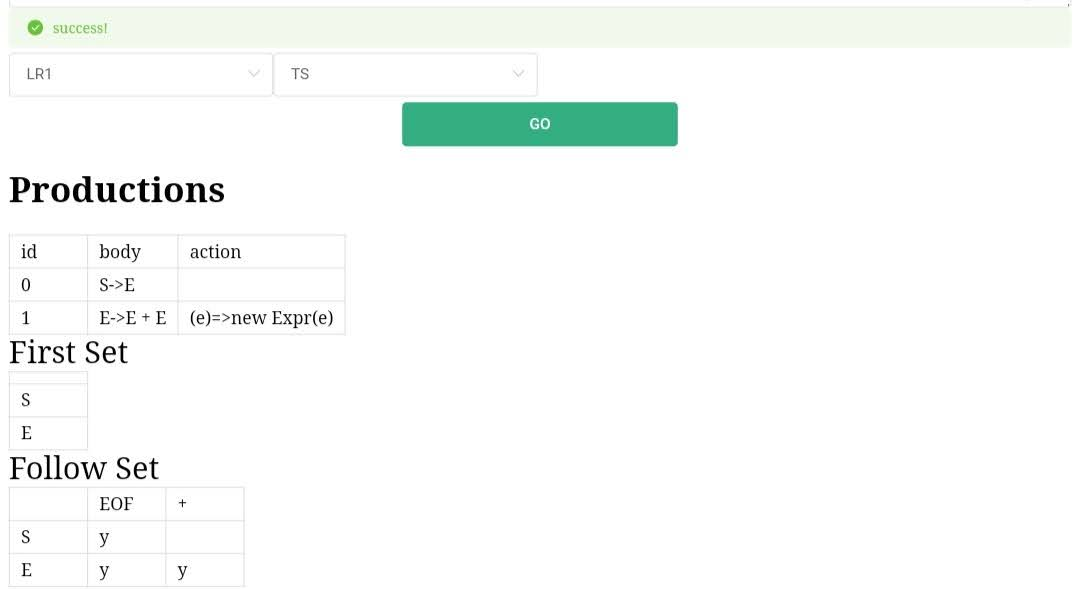
\includegraphics[width=15.6cm]{figuras/lightparsers2.jpg
%     }}{\Fonte{\textcite{Parser-2024-04-12}.}}
% \end{figure}

% \section{LR(1) \textit{Parser Generator}}
% Feita especificamente para o algoritmo CLR a ferramenta \textit{web} criada por \textcite{LR-2024-04-12} gera o conjunto de \textit{first} mostrado na Figura \ref{fig:firstandcanonical}, o conjunto de itens canônicos mostrado na Figura \ref{fig:firstandcanonical} e a tabela de transição de estados mostrada na Figura \ref{fig:tableandparse}. A ferramenta também disponibiliza o passo a passo da análise de uma \textit{string} junto com uma árvore sintática representada por contêineres contidos um dentro do outro como mostra a Figura \ref{fig:tableandparse}.

% \begin{figure}[ht]
%     \captionsetup{width=16cm}
%     \Caption{\label{fig:tableandautomata}Imagem da ferramenta de \textit{Parser Generator Web Tools}}
%     \tcbox[left=0cm, right=0cm, top=0cm, bottom=0cm,center]{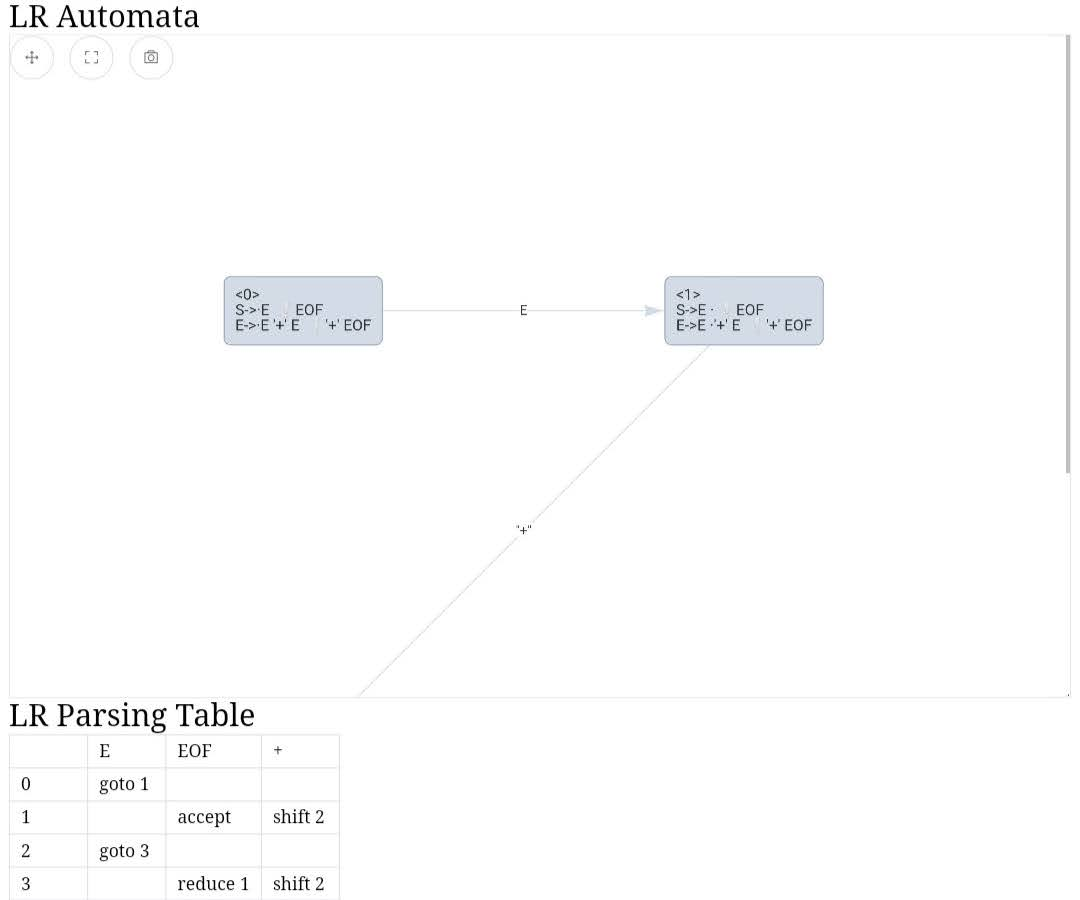
\includegraphics[width=15.6cm]{figuras/lightparsers.jpg}}
%     {\Fonte{\textcite{Parser-2024-04-12}.}}
% \end{figure}

% \begin{figure}[ht]
%     \captionsetup{width=16cm}
%     \Caption{\label{fig:firstandcanonical}Imagem da ferramenta de LR(1) \textit{Parser Generator}}
%     \tcbox[left=0cm, right=0cm, top=0cm, bottom=0cm,center]{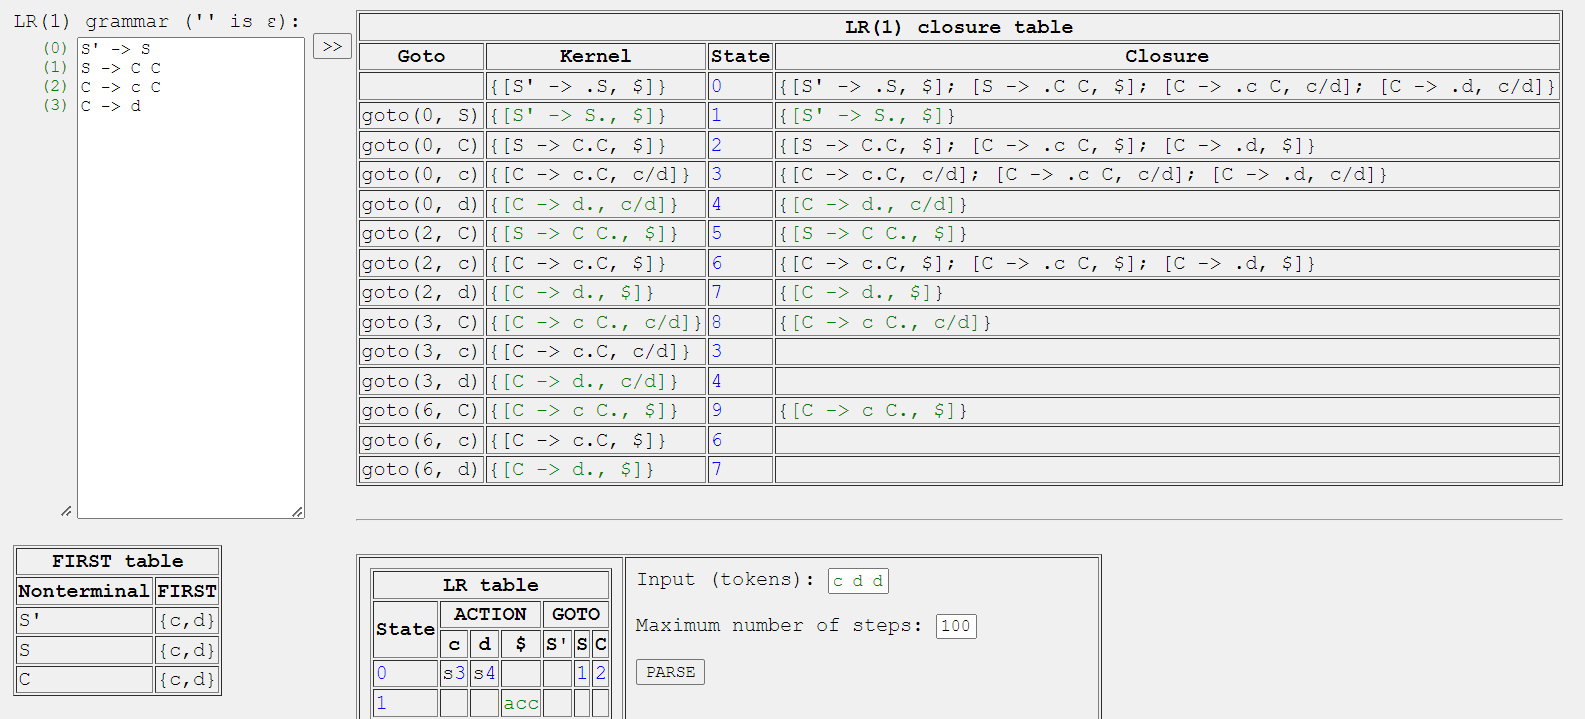
\includegraphics[width=15.6cm]{figuras/lrparser2.png}}{
%     \Fonte{\textcite{LR-2024-04-12}.}}
% \end{figure}

% \begin{figure}[ht]
%     \captionsetup{width=16cm}
%     \Caption{\label{fig:tableandparse}Imagem da ferramenta de LR(1) \textit{Parser Generator}}
%     \tcbox[left=0cm, right=0cm, top=0cm, bottom=0cm,center]{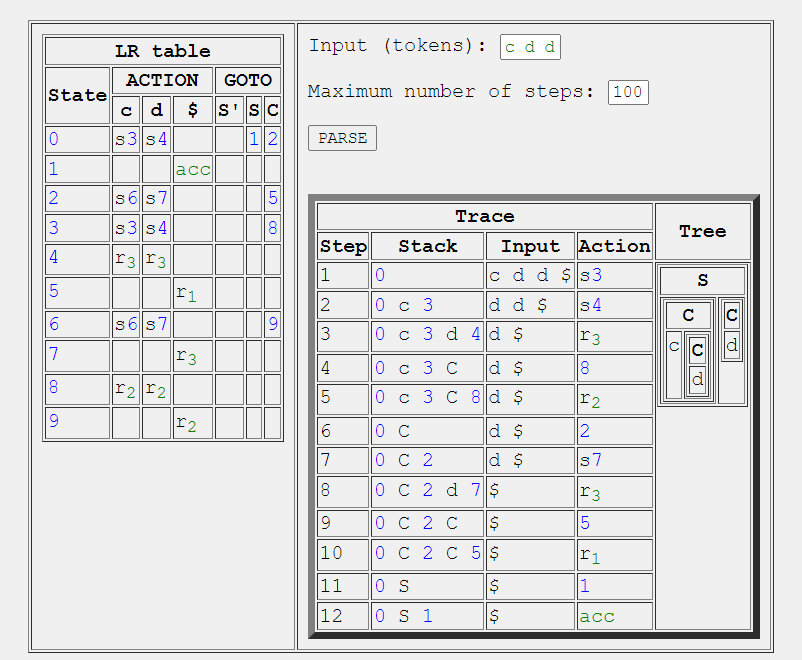
\includegraphics[width=15.6cm]{figuras/lrparser.png}}{
%     \Fonte{\textcite{LR-2024-04-12}.}}
% \end{figure}
%\FloatBarrier

\section{\textit{PAVT: a tool to visualize and teach parsing algorithms}}
No trabalho de \textcite{sangal2018pavt} foi introduzida a ferramenta PAVT com o objetivo de ensinar seis algoritmos de análise sintática. Os algoritmos que são abordados na ferramenta são \textit{predictive parsing}, \textit{simple LR (SLR) parsing}, \textit{canonical LR(CLR) parsing}, \textit{look-ahead LR(LALR) parsing}, \textit{earley parsing e Cocke-Younger-Kasami(CYK) parsing}. PAVT mostra uma breve descrição dos algoritmos e dá o resultado dos passos do algoritmo em formato de texto. Para utilizar a ferramenta o usuário deve digitar uma string para ser analisada e a gramática alvo ou fazer upload de um arquivo de texto contendo a gramática. A interface da ferramenta pode ser vista na Figura \ref{fig:pavt}.
\begin{figure}[h]
    \captionsetup{width=16cm}
    \Caption{\label{fig:pavt}Interface da ferramenta PAVT}
    \tcbox[left=0cm, right=0cm, top=0cm, bottom=0cm,center]{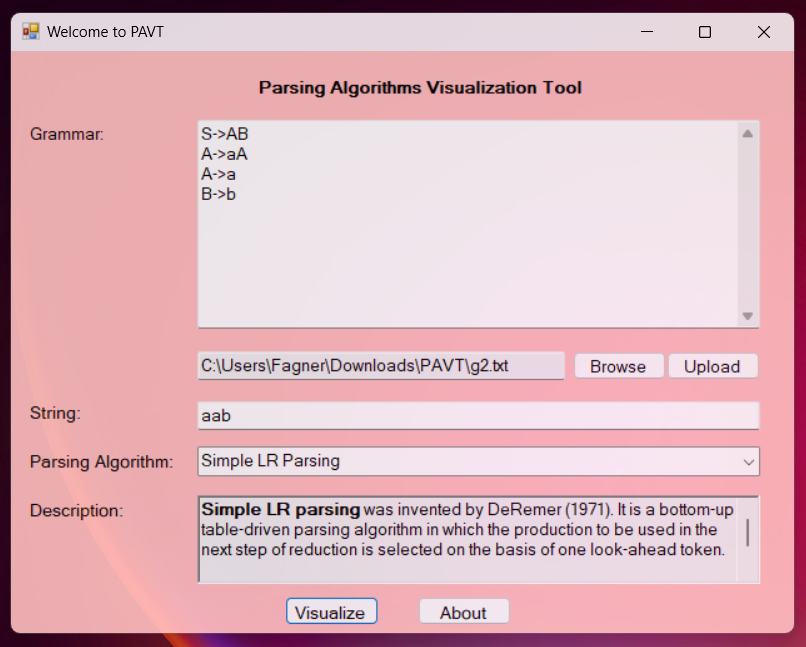
\includegraphics[width=15.6cm]{figuras/pavt.png}}{
    \Fonte{adaptada de \textcite{pavt}.}}
\end{figure}

PAVT tem módulos que são responsáveis pela visualização de cada algoritmo. Para todos é feita a análise da string de entrada, caso a string seja aceita é construída a árvore sintática representada da esquerda para direita. Além disso, todos os elementos presentes nos algoritmos são apresentados, esses elementos são o conjunto first, conjunto follow, conjunto de itens, tabela de parsing e derivação mais à direita.

A ferramenta foi usada no curso de construção de compiladores e ao fim do curso o \textit{feedback} dos alunos foi coletado. Os resultados obtidos indicaram que a ferramenta ajudou no aprendizado de algoritmos de análise sintática, os autores afirmam que os resultados de cada passo dos algoritmos são dados em um formato comumente usado pelos professores e ajudam os estudantes a praticar e entender os algoritmos.


% \section{PAVT}
% No trabalho de \textcite{sangal2018pavt} foi criada a ferramenta PAVT (\textit{Parsing Algorithms Visualization Tool}) para visualização de seis algoritmos de análise sintática. A ferramenta apresenta uma caixa de entrada para informar a gramática a opção de importar uma gramática através de um arquivo, uma caixa de entrada para as \textit{string} a serem analisadas e uma breve descrição dos algoritmos disponíveis. Todos os elementos da ferramenta podem ser vistos na Figura \ref{fig:pavt}. Apesar da ferramenta oferecer a visualização dos algoritmos, essa visualização é realizada apenas pela leitura de um arquivo de texto gerado pela ferramenta, além de não mostrar instruções de como chegar ao resultado descrito no arquivo de texto. O \textit{software} também está apenas disponível em versão \textit{desktop} para o sistema operacional \textit{Windows}.

\section{\textit{A Web-Based Educational System for Teaching Compilers}}
O trabalho de \textcite{webbased} foi feito na universidade de Pristina com o objetivo de criar uma versão \textit{web} de um sistema de simulação ComVis, um sistema com módulos que ensinam as fases da compilação. O sistema já havia sido desenvolvido em Java para \textit{desktop}, no entanto, por questões de acessibilidade e melhor representação visual foi decidido criar a versão \textit{web} do sistema. A motivação por trás desse trabalho foi a dificuldade dos alunos da universidade na disciplina de compiladores. Os autores também citam como a utilização de um software interativo pode ajudar na motivação.

O sistema foi desenvolvido usando \textit{Java Server Page}, já que a versão \textit{desktop} do sistema foi feita em Java, grande parte da base de código pôde ser reutilizada dessa forma. Outras tecnologias usadas foram HTML, CSS, JavaScript e Graphviz para criação de gráficos e diagramas.

No estudo foi feita uma análise comparativa entre as versões \textit{web} e \textit{desktop} do sistema. A partir dessa análise os autores concluíram que a versão \textit{web} criada tem melhor acessibilidade, visualização, controle da simulação e \textit{feedback}. Também foi feita uma avaliação quantitativa da eficiência do sistema, os resultados mostram que os estudantes que usaram o sistema tiveram melhor desempenho do que aqueles que não usaram o sistema.


\section{\textit{A Tool for Visualization of Parsers: JFLAP}}
JFLAP (\textit{Java Formal Languages and Automata Package}) é uma ferramenta \textit{desktop} criada por \textcite{jflap} primariamente para a construção e simulação de autômatos e gramáticas livres de contexto. O trabalho de \textcite{jflapparser} introduz os algoritmos LL(1) e SLR na ferramenta, dessa forma, JFLAP também pode ser usado para visualização dos algoritmos LL(1), SLR e de força bruta. Como mostra a Figura \ref{fig:jflap}, a ferramenta apresenta os conjuntos \textit{first} e \textit{follow}, o autômato dos estados do analisador sintático e a tabela de ações. O processo de \textit{parsing} também é disponibilizado assim como a árvore sintática.

\begin{figure}[h]
    \captionsetup{width=16cm}
    \Caption{\label{fig:jflap}Imagem da ferramenta JFLAP}
    \tcbox[left=0cm, right=0cm, top=0cm, bottom=0cm,center]{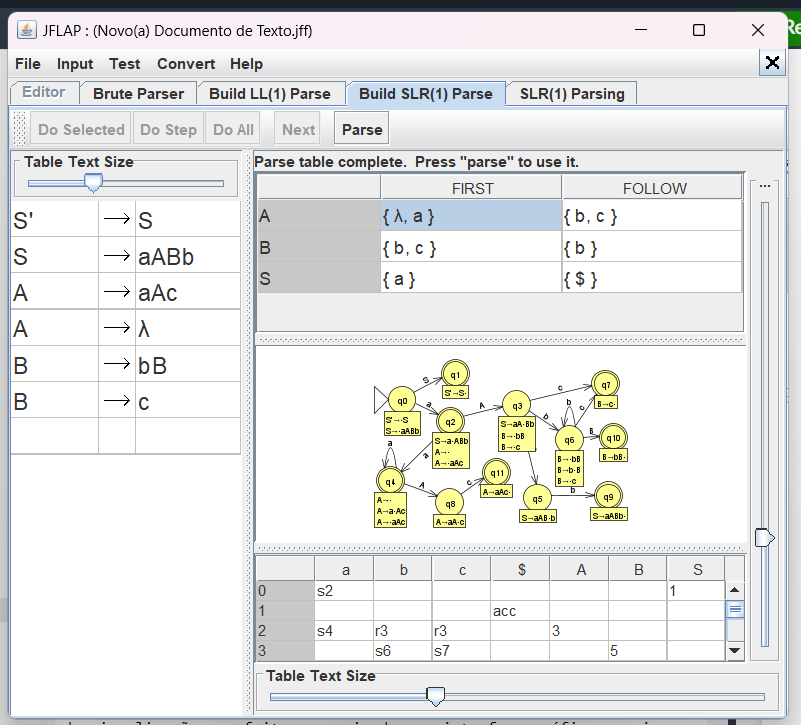
\includegraphics[width=15.6cm]{figuras/jflap.png}}{
    \Fonte{\textcite{jflap}.}}
\end{figure}

\section{Considerações}
Apesar de já existirem ferramentas de visualização de \textit{parsers}, algumas desvantagens ainda precisam ser consideradas. Uma limitação é que o conteúdo não tem muita interatividade, a ferramenta apresentada no trabalho de \textcite{sangal2018pavt}, por exemplo, apresenta apenas em um arquivo de texto. Isso pode dificultar a compreensão dos conceitos. Outra limitação é a falta de detalhamento do passo a passo dos algoritmos, por exemplo a ferramenta apresentada no trabalho de \textcite{webbased} foca apenas no último passo da análise sintática, excluindo a parte de construção das tabelas de \textit{parsing} e conjuntos de itens. Isso impede que os estudantes acompanhem o funcionamento interno dos processos de análise. Por fim, nenhuma das ferramentas apresenta uma versão \textit{mobile}. Essas lacunas representam oportunidades de melhoria para que as ferramentas de visualização de \textit{parsers} se tornem ainda mais eficazes no apoio ao ensino e aprendizagem de análise sintática. No Quadro \ref{qua:comparativo} pode-se ver o resumo do comparativo dos trabalhos citados anteriormente.

\setlength{\abovecaptionskip}{10pt plus 0pt minus 0pt}
\setlength{\belowcaptionskip}{5pt plus 0pt minus 0pt}
\begin{table}[h]
\centering\setlength{\extrarowheight}{2pt}
\captionsetup{width={\textwidth}}
\captionof{quadro}{Comparativo de trabalhos relacionados}\label{qua:comparativo}
\resizebox{\textwidth}{!}{\begin{NiceTabular}{l*{7}{c}}[corners,hvlines]
\CodeBefore
  \rowcolor{gray!15}{1-2}
\Body
\Block{2-1}{Trabalho}&\Block{1-3}{Algoritmos}&&&\Block{1-3}{Plataformas}&&&\Block{2-1}{Integração com Moodle}\\

&LL(1)&SLR&CLR&Mobile&Desktop&Web\\
\textcite{munozquestions}                   &x&x& & & &x\\
\textcite{sangal2018pavt}                   & &x&x& &x& \\
\textcite{webbased}                         & &x&x& &x&x\\
\textcite{jflapparser}                      &x&x& & &x& \\
Este trabalho &x&x&x&x&x&x&x \\
\end{NiceTabular}}
{\Fonte{fornecido pelo autor}}
\end{table}




% \begin{figure}[t!]
%     \captionsetup{width=16cm}
%     \Caption{\label{fig:jflapparse}Imagem da ferramenta JFLAP}
%     \tcbox[left=0cm, right=0cm, top=0cm, bottom=0cm,center]{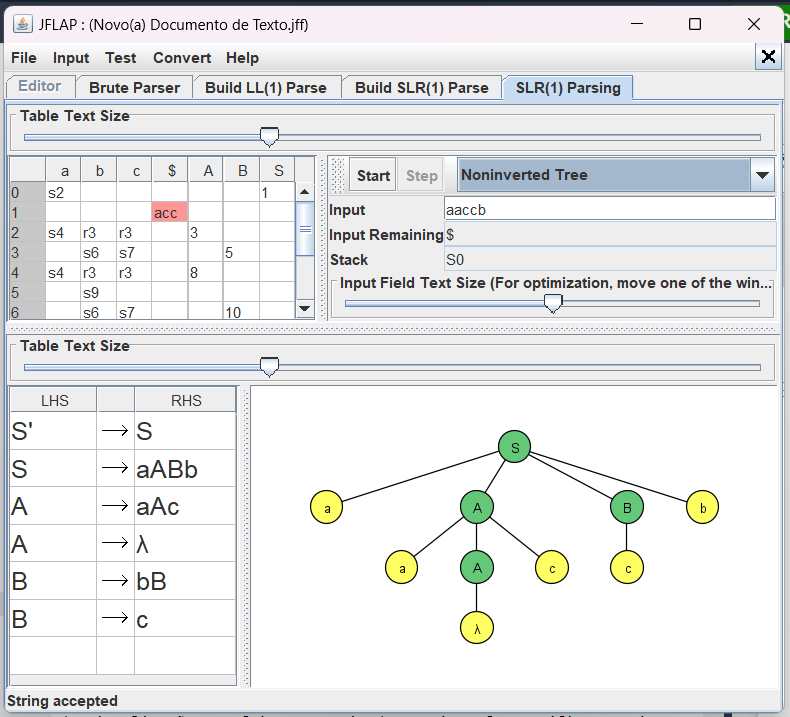
\includegraphics[width=15.6cm, height=7.85cm]{figuras/jflapparse.png}}{
%     \Fonte{\textcite{jflap}.}}
% \end{figure}
%\FloatBarrier

	\chapter{Metodologias}
\label{chap:metodologia}
Nesta seção serão apresentadas as metodologias usadas para o desenvolvimento desse trabalho. As etapas a serem seguidas estão representadas no fluxograma da Figura \ref{fig:etapas}.

\begin{figure}[ht]
  \centering
  \captionsetup{width=16cm}
  \caption{Fluxograma das etapas}
  \label{fig:etapas}
  \tcbox[left=0cm, right=0cm, top=0cm, bottom=0cm,center]{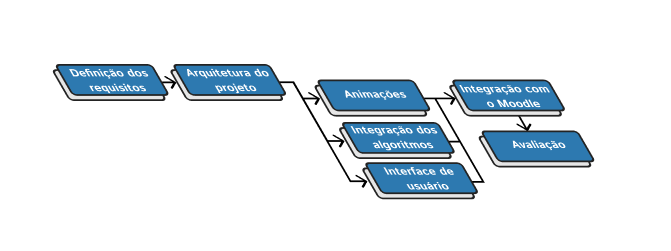
\includegraphics[width=15.6cm]{figuras/fluxograma.png}}
  \Fonte{fornecida pelo próprio autor}
\end{figure}

\section{Definir os requisitos}
A partir da revisão bibliográfica foram definidos alguns requisitos básicos que deveriam estar presentes na ferramenta. Como requisito não funcional foi definido oferecer suporte multi-plataforma, para \textit{mobile}, \textit{desktop} e \textit{web}. Como requisitos funcionais foram definidos os seguintes:
\begin{itemize}[label={$\sbullet$}]
  \item Permitir que os usuários digitem a gramática a ser analisada.
  \item Permitir que os usuários visualizem o estado das estruturas dos algoritmos.
  \item Permitir que os usuários avancem, retornem e reiniciem os passos da execução dos algoritmos.
  \item Permitir que os usuários selecionem o algoritmo a ser visualizado.
\end{itemize}

Apesar das ferramentas compartilharem as mesmas funcionalidades básicas já definidas inicialmente, outras têm características interessantes que podem ser reaproveitadas, partir delas foram definidos os seguintes requisitos:
\begin{itemize}[label={$\sbullet$}]
  \item Permitir que os usuários digitem uma \textit{string} a ser analisada.
  \item Permitir que os usuários visualizem a análise de uma \textit{string}.
  \item Permitir que os usuários visualizem a árvore sintática de uma \textit{string}.
  \item Permitir que os usuários copiem em formato de texto os resultados da análise de uma \textit{string}.
  \item Permitir que os usuários copiem implementações dos algoritmos.
\end{itemize}

Com esses requisitos tem-se a base para o desenvolvimento da ferramenta.

\section{Definir a arquitetura do projeto}
O projeto será construído usando o \textit{framework Svelte}, sem \gls{ssr}, para que seja possível o funcionamento \textit{offline} da ferramenta, já que a ferramenta não teria acesso ao servidor não seria possível usá-lo para renderizar elementos. \textit{Svelte} compila a base de código e cria uma coleção de arquivos estáticos que constituem a página \textit{web} e a base para o suporte multi-plataforma da aplicação.
\begin{figure}[ht]
  \centering
  \captionsetup{width=16cm}
  \caption{Arquitetura da aplicação em nuvem}
  \label{fig:arqremo}
  \tcbox[left=0cm, right=0cm, top=0cm, bottom=0cm,center]{
    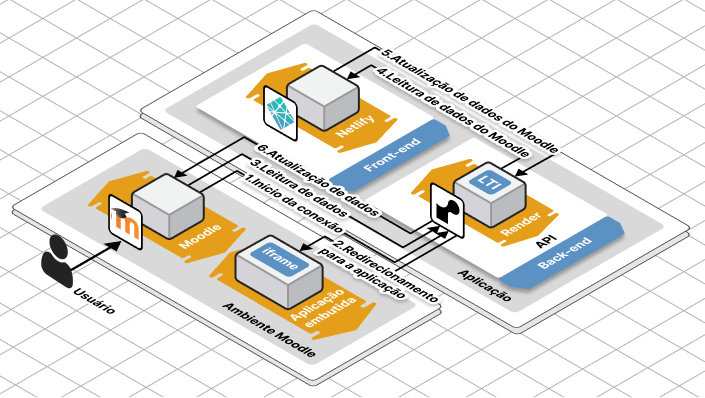
\includegraphics[width=15.6cm]{figuras/remote.png}}
  \Fonte{fornecida pelo próprio autor}
\end{figure}

O \textit{framework Capacitor} consome essa coleção de arquivos e cria um projeto para plataforma \textit{Android} que é usado para criar a versão \textit{mobile} da ferramenta usando o \textit{Android Studio}. O \textit{framework Tauri} constrói instaladores para \textit{desktop} diretamente da coleção de arquivos estáticos. A plataforma alvo dos instaladores é a plataforma na qual eles são construídos, já que o \textit{framework} não tem suporte para construção \textit{cross-platform} é necessária a utilização de máquinas virtuais para construir instaladores para diferentes plataformas \textit{desktop}.

Para a versão \textit{online} da aplicação, os serviços de computação em nuvem das empresas \textit{Netlify} e \textit{Render} serão usados para hospedar respectivamente o \textit{front-end} e \textit{back-end} da aplicação. \textit{Netlify} e \textit{Render} foram escolhidas para hospedagem da aplicação pelo oferecimento gratuito dos serviços para aplicações pequenas como a proposta nesse trabalho.

A aplicação pode ser acessada através do \textit{Moodle} usando como comunicação entre os dois a \gls{api} da aplicação. O diagrama na Figura \ref{fig:arqremo} mostra o esquema da arquitetura da aplicação hospedada em nuvem com integração ao \textit{Moodle}. A versão hospedada localmente da aplicação segue a mesma arquitetura com exceção da utilização de serviços de computação em nuvem.


%\FloatBarrier

\section{Implementar a interface de usuário}
Para que o usuário selecione um algoritmo para visualizar a ferramenta terá opções no topo da tela que alternam entre abas. Dentre essas abas estarão inclusas uma para a entrada de gramáticas e uma aba para visualização de cada algoritmo disponível. Para que o usuário possa dar uma gramática de entrada será criado um campo de texto como mostra Figura \ref{fig:mgrammar}.

\begin{figure}[ht]
  \centering
  \captionsetup{width=16cm}
  \caption{Aba de entrada da gramática}
  \label{fig:mgrammar}
  \tcbox[left=0cm, right=0cm, top=0cm, bottom=0cm,center]{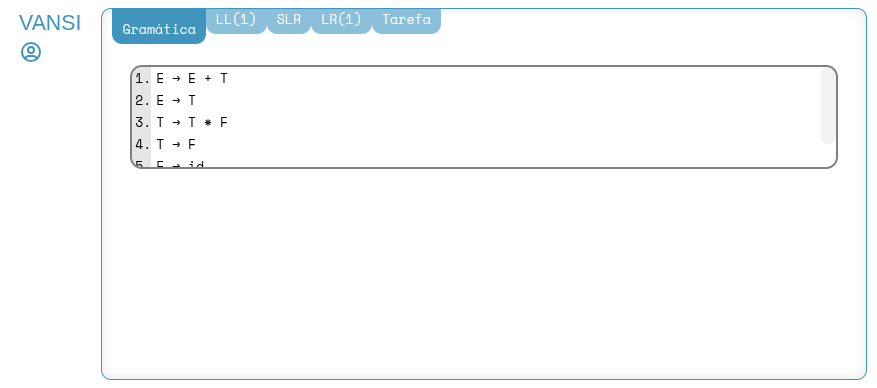
\includegraphics[width=15.6cm]{figuras/mgrammar.png}}
  \Fonte{fornecida pelo próprio autor}
\end{figure}

Para a visualização dos algoritmos a ferramenta terá uma composição de elementos como mostra a Figura \ref{fig:mfirst}, esses elementos são modificados de acordo com a execução do algoritmo selecionado. Os passos da execução do algoritmo podem ser controlados pelo conjunto de controles acima dos elementos do algoritmo como mostra a Figura \ref{fig:mfirst}.

\begin{figure}[ht]
  \centering
  \captionsetup{width=16cm}
  \caption{Aba de visualização dos algoritmos}
  \label{fig:mfirst}
  \tcbox[left=0cm, right=0cm, top=0cm, bottom=0cm,center]{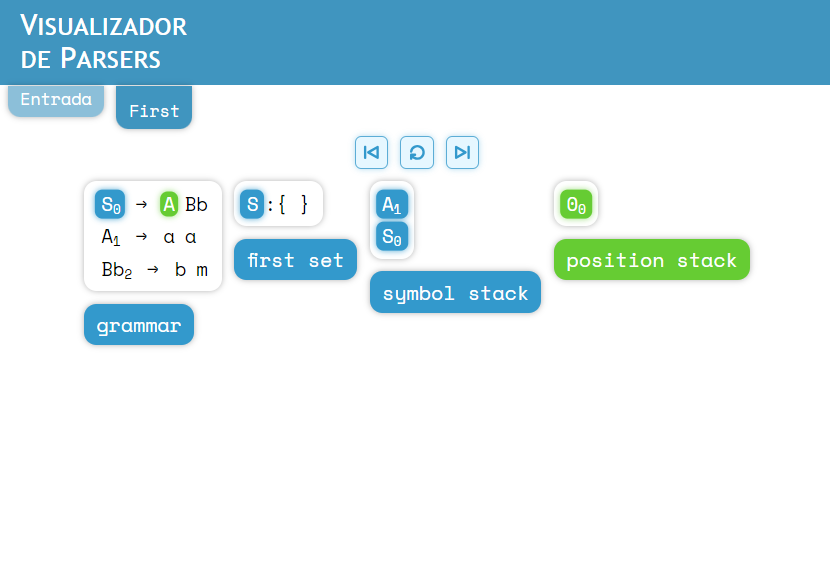
\includegraphics[width=15.6cm]{figuras/mfirst.png}}
  \Fonte{fornecida pelo próprio autor}
\end{figure}

Nas abas de visualização de algoritmos serão inclusos um campo de texto no qual o usuário poderá inserir uma \textit{string} de entrada para ser analisada pelo algoritmo, um campo de texto para copiar os resultados dos algoritmos em forma de texto e um campo de texto para copiar a implementação do algoritmo.

\section{Integrar os algoritmos à ferramenta}
Para todas as estruturas de dados usadas nos algoritmos serão criadas representações visuais, dessa forma todos os passos do funcionamento poderão ser representados como estados dessas estruturas. Calculando antecipadamente os estados dessas estruturas em cada passo dos algoritmos podemos fazer um controle de fluxo entre os passos dos algoritmos.

\section{Implementar as animações dos algoritmos}
As mudanças de estados que ocorrem nos algoritmos podem ser melhor compreendidas se poderem ser visualizadas como transições ao invés de mostrar as mudanças saltando do estado inicial para o estado final. Usar animações torna a visualização das mudanças muito mais dinâmica. Um exemplo de animação é a animação do estado da estrutura de pilha que é usada em alguns algoritmos. Quando um item é adicionado ou removido da pilha, o elemento visual que representa esse item terá sua posição interpolada do ponto inicial ao ponto final.

\section{Integrar a ferramenta com o \textit{Moodle}}
A plataforma \gls{lms} \textit{Moodle} implementa o padrão \gls{lti} o que permite a utilização da ferramenta criada nesse trabalho diretamente no \textit{Moodle} sem necessidade de \textit{login} externo. Para que a ferramenta possa utilizar o padrão \gls{lti} com o \textit{Moodle} será implementado no \textit{back-end} da aplicação uma \gls{api} que manuseia as requisições relacionada ao \gls{lti}.

Os \textit{endpoints} da \gls{api} foram definidos de acordo com o Quadro \ref{qua:endpoints}.

\setlength{\abovecaptionskip}{10pt plus 0pt minus 0pt}
\setlength{\belowcaptionskip}{5pt plus 0pt minus 0pt}
\begin{table}[h]
  \centering\setlength{\extrarowheight}{2pt}
  \captionsetup{width={\textwidth}}
  \captionof{quadro}{Endpoints}\label{qua:endpoints}
  \resizebox{\textwidth}{!}{
    \begin{NiceTabular}{m[c]{3cm}m[c]{3cm}m[c]{10cm}}[corners,hvlines]
      \CodeBefore
      \rowcolor{gray!15}{1-1}
      \Body
      \textbf{Endpoint}                                                  & \textbf{Método} & \textbf{Finalidade}                 \\
      \selectlanguage{brazil}$\backslash$\selectlanguage{brazil}         & GET             & redirecionar para página            \\
      \selectlanguage{brazil}$\backslash$\selectlanguage{brazil}login    & POST            & inicia uma conexão com a plataforma \\
      \selectlanguage{brazil}$\backslash$\selectlanguage{brazil}register & POST            & registrar uma nova plataforma       \\
    \end{NiceTabular}}
  {\Fonte{fornecido pelo autor}}
\end{table}

Com a \gls{api} pronta pode ser feita a conexão entre a ferramenta e a \gls{lms}. Utilizando o serviço \gls{lti} de \textit{Dynamic Registration} é possível fazer o cadastro da ferramenta no \textit{Moodle} utilizando um \textit{link} para o \textit{endpoint} de registro dinâmico da \gls{api}.

\section{Avaliar a ferramenta}
Será realizado um teste prático com um grupo de estudantes, onde os eles serão solicitados a realizar tarefas específicas utilizando a ferramenta. Serão coletados dados quantitativos, como tempo de execução das tarefas e taxa de acerto, bem como dados qualitativos por meio de questionários e entrevistas para avaliar a percepção dos estudantes sobre a eficácia da ferramenta. Além disso, a comparação dos resultados obtidos com um grupo de controle que não utiliza a ferramenta ajudará a avaliar o impacto da visualização na compreensão e desempenho dos alunos. Essa abordagem abrangente de avaliação garantirá uma análise completa da eficácia e utilidade da ferramenta desenvolvida nesse trabalho.

O desenvolvimento desse trabalho seguirá o cronograma mostrado no Quadro \ref{qua:cronograma}.
\setlength{\abovecaptionskip}{10pt plus 0pt minus 0pt}
\setlength{\belowcaptionskip}{5pt plus 0pt minus 0pt}
\begin{table}[h]
  \centering\setlength{\extrarowheight}{2pt}
  \captionsetup{width={\textwidth}}
  \captionof{quadro}{Cronograma}\label{qua:cronograma}
  \resizebox{\textwidth}{!}{\begin{NiceTabular}{l*{6}{c}}[corners,hvlines]
      \CodeBefore
      \rowcolor{gray!15}{1-3}
      \Body
      \Block{3-1}{Atividades}             & \Block{1-6}{Período}                                                               \\
                                          & \Block{1-3}{2024}    &          &          & \Block{1-3}{2025}                     \\
                                          & Outubro              & Novembro & Dezembro & Janeiro           & Fevereiro & Março \\

      Definir dos requisitos              & x                    &          &          &                   &           &       \\
      Definir arquitetura do projeto      & x                    &          &          &                   &           &       \\
      Implementar da interface de usuário &                      & x        & x        &                   &           &       \\
      Integrar os algoritmos              &                      &          & x        & x                 & x         &       \\
      Implementar as animações            &                      &          & x        & x                 & x         &       \\
      Integrar ao Moodle                  &                      &          &          & x                 & x         &       \\
      Avaliar a ferramenta                &                      &          &          &                   & x         &       \\
      Escrita do TCC II                   & x                    & x        & x        & x                 & x         & x     \\
      Defesa do TCC II                    &                      &          &          &                   &           & x     \\
    \end{NiceTabular}}
  {\Fonte{fornecido pelo autor}}
\end{table}

	% \input{2-textuais/5-resultados}
	%\input{2-textuais/6-conclusao}
	%\printglossary
    
	%Elementos pós-textuais
    %\bibliographystyle{lib/abntex2-alf}
	% \bibliography{3-pos-textuais/referencias}
	\nocite{*} 
	\urlstyle{same}
	\begin{SingleSpace}
	\printbibliography
	\end{SingleSpace}
            
	%\printglossary
	%\imprimirglossario 
	% \imprimirapendices
		% Adicione aqui os apendices do seu trabalho
		%\apendice{EXEMPLO DE APÊNDICE}
\label{ap:A}

Um apêndice é um documento elaborado pelo autor, diferentemente do anexo. Geralmente, se coloca como apêndice, questionários, códigos de programação, tabelas que tomariam muito espaço no meio do trabalho.
		%\apendice{ Questionário utilizado para}
\label{ap:B}

\begin{questao}
	\item Esta é a primeira questão com alguns itens:
		\begin{enumerate}
			\item Este é o primeiro item
			\item Segundo item
		\end{enumerate}
	\item Esta é a segunda questão:
		\begin{enumerate}
			\item Este é o primeiro item
			\item Segundo item
		\end{enumerate}
	\item Lorem ipsum dolor sit amet, consectetur adipiscing elit. Nunc dictum sed tortor nec viverra. consectetur adipiscing elit. Nunc dictum sed tortor nec viverra.
		\begin{enumerate}
			\item consectetur
			\item adipiscing
			\item Nunc
			\item dictum
		\end{enumerate}
\end{questao}

		%\apendice{ Códigos-fontes utilizados para}
\label{ap:C}

\lstinputlisting[language=C++,caption={Hello World em C++}]{figuras/main.cpp}


\begin{lstlisting}[language=Java,caption={Hello World em Java}]
public class HelloWorld {
	public static void main(String[] args) {
		System.out.println("Hello World!");
	}
}
\end{lstlisting}


		
		% \imprimiranexos
		% Adicione aqui os anexos do seu trabalho
		% \anexo{ Exemplo de um anexo}
\label{an:ex_anexo_a}

Um anexo é um documento que não foi elaborado pelo autor, ou seja, o autor apenas anexa. Anexos podem ser tabelas, mapas, diagramas, \textit{datasheets}, manuais e etc. 




		% \anexo{ Exemplo de um anexo em PDF}
\label{an:ex_anexo_b}

O autor pode anexar um \gls{PDF}, traduzido como formato portátil de documento. Veja o código fonte utilizado para anexar o arquivo ``Sikasil.pdf'' que foi colocado dentro da pasta ``anexos'' que por sua vez está dentro da pasta ``elementos-pos-textuais''. Tenha muita atenção na hora de especificar o local do arquivo. Recomenda-se não utilizar caracteres especiais para nomear pastas e, principalmente, arquivos. 

Pode-se fazer uma descrição sucinta do arquivo anexado.

%Comando para incluir um arquivo em PDF:
% \includepdf[pages={-}]{3-pos-textuais/anexos/Sikasil.pdf}

		
    %\imprimirindice
    
	

\end{document}